\documentclass[conference]{IEEEtran}
\usepackage{amsmath,amssymb}
\usepackage{booktabs}
\usepackage{graphicx}
\usepackage{subcaption}
\usepackage{hyperref}

\begin{document}

\title{Fixed-K Speculative Decoding for Energy-Proportional LLM Serving: \\
A Reproducible Empirical Validation}

\author{
\IEEEauthorblockN{Zanno Jacklin}
\IEEEauthorblockA{Independent Researcher, Creepybits}
}

\maketitle

\begin{abstract}
We present an empirical validation of fixed draft-length ($K{=}5$) speculative
decoding using a scout(1B)$\to$target(8B) model pair on consumer GPU hardware.
Across three prompt categories spanning low to high output determinism (creative
poetry, technical explanation, and code generation), we measure throughput,
energy per token, and output fidelity relative to a matched FP16 autoregressive
baseline. Speculative decoding achieves up to +82.3\% throughput
improvement and $-$60.3\% energy reduction per token on
code generation, with smaller but consistent gains on less predictable prose
(+8.6\% / $-$32.6\% on poetry). All results
achieve 100\% exact-token-match fidelity against the baseline (lossless,
greedy decoding) and are independently reproducible from the accompanying
open-source repository. We report results transparently, including the
deliberate methodological choice to omit KV-caching from both arms of the
comparison, which keeps the relative comparison fair but means absolute
throughput figures are not representative of a production-optimized server.
\end{abstract}

\begin{IEEEkeywords}
speculative decoding, energy-efficient inference, large language models, GPU power measurement
\end{IEEEkeywords}

\section{Introduction}

Autoregressive decoding in large language models (LLMs) is inherently
sequential: each output token requires a full forward pass through the
target model before the next token can be produced. This serial dependency
underutilizes modern GPU compute, which is optimized for parallel throughput.
Speculative decoding~\cite{leviathan2023fast,chen2023accelerating} addresses
this by using a smaller, faster \emph{scout} model to propose a short window
of candidate tokens, which the larger \emph{target} model then verifies in a
single parallel forward pass, accepting the longest correct prefix.

This paper reports a narrow, fully-validated empirical claim: a fixed draft
window of $K{=}5$ tokens, paired with an exact (lossless) accept/reject
verification scheme, produces measurable throughput and energy improvements
on real consumer GPU hardware, with perfect output fidelity relative to
standard greedy decoding. We deliberately scope this paper to only the
mechanism we have fully validated. A related, more ambitious mechanism
under investigation in the parent project --- entropy-gated \emph{dynamic}
adjustment of the draft window, intended to switch between aggressive and
conservative speculation based on local output entropy --- is explicitly
\textbf{not} included here, as it has not yet been shown to outperform this
simpler fixed-$K$ approach in single-request testing.

\subsection{Relationship to prior work}

Entropy-gated adaptive speculative decoding is an active research area.
AdaEDL~\cite{adaedl2024} reports 10--57\% improvement over static draft
length using entropy-based adaptive drafting. SGLang ships a built-in
adaptive speculative-length mechanism using an EMA of accepted draft length.
Our own testing of an entropy-gated variant, using the same hardware and
methodology as this paper, has not yet demonstrated an improvement over the
simpler fixed-$K$ approach reported here; we regard that as an open question
requiring further work (e.g. testing under multi-request/batched serving,
which published entropy-gating results suggest is where the technique's
value proposition may actually lie), not a settled negative result. This
paper makes no claims about the entropy-gated mechanism in either direction.

\section{Methodology}

\subsection{Models and hardware}

Scout model: Llama-3.2-1B-Instruct. Target model: Llama-3.1-8B-Instruct.
Both loaded in bfloat16. All measurements taken on a single NVIDIA RTX 5090
(Blackwell architecture) GPU, single-request (batch size 1), greedy
(argmax) decoding throughout.

\subsection{Draft-verify procedure}

At each decoding cycle, the scout model autoregressively proposes $K{=}5$
candidate tokens. The target model then performs a single forward pass over
the full draft sequence, and its argmax predictions at each position are
compared against the corresponding drafted tokens. The longest matching
prefix is accepted; at the first mismatch (or after all $K$ tokens match),
the target's own prediction is substituted, exactly reproducing what
standard greedy decoding would have produced at that position. This
verification scheme is lossless by construction: the output token sequence
is provably identical, position-for-position, to what running the target
model alone would produce, since every emitted token is either a drafted
token confirmed by the target's own argmax, or the target's argmax directly.

\subsection{Power and energy measurement}

GPU power is sampled via NVML at 100~Hz on a background thread throughout
each timed generation window. Energy per token is computed as
$E_{\text{tok}} = \bar{P} \cdot t / N_{\text{tok}}$, where $\bar{P}$ is mean
sampled power over the generation window, $t$ is wall-clock generation time,
and $N_{\text{tok}}$ is the number of tokens produced.

\subsection{Warmup}

Both the baseline and speculative measurement paths are preceded by 5
untimed forward-pass warmup steps immediately before each timed trial. This
avoids attributing CUDA kernel compilation and GPU clock ramp-up latency to
the measured region. This warmup procedure is applied identically to both
arms of the comparison.

\subsection{Deliberate exclusion of KV-caching}

Both the baseline and speculative decoding paths recompute attention over
the full sequence at every step, with no KV-cache reuse. This was a
deliberate methodological choice: an earlier iteration of this work applied
caching only to the baseline arm, which structurally penalized the
speculative path whenever it fell back to single-step generation (a full
uncached recompute for a single token is the worst-case cost ratio in the
system). Removing caching from both arms restores a fair relative
comparison at the cost of both arms being substantially slower in absolute
terms than a production server with caching would be. We therefore report
\emph{relative} throughput and energy figures as the validated result, and
explicitly flag that absolute tok/s numbers in this paper are not
production-representative.

\subsection{Fidelity measurement}

Fidelity is measured as the exact token-for-token match rate between the
baseline's greedy output and the speculative path's output, over the full
generated sequence, for each prompt.

\subsection{Prompts}

Three prompts were selected to span a range of output determinism:
\begin{itemize}
\item \textbf{Poem} (low determinism): an open-ended creative writing task
(an original Chant Royal poem on a mathematical theme).
\item \textbf{Physics} (medium determinism): a technical explanation task
(semiconductor memory bandwidth and the memory wall).
\item \textbf{Code} (high determinism): a code-generation task (a Python
binary search tree implementation with type annotations), where correct
completions are far more constrained token-to-token.
\end{itemize}

\section{Results}

\subsection{Fidelity}

Aggregate exact-token-match fidelity across all three prompts was
100.0\%, confirming the accept/reject implementation is lossless
in practice as well as by construction.

\subsection{Throughput, energy, and power}

Table~\ref{tab:results} reports mean $\pm$ standard deviation across
$N{=}10$ trials per prompt per condition.

\begin{table*}[t]
\centering
\caption{Baseline vs. fixed-$K{=}5$ speculative decoding, per prompt. N=10 trials/prompt.}
\label{tab:results}
\begin{tabular}{lccccccc}
\toprule
Prompt & Baseline tok/s & Spec. tok/s & Speedup & Baseline J/tok & Spec. J/tok & Energy $\Delta$ & Accept \% \\
\midrule
Poem     & 40.0 $\pm$ 0.62 & 43.4 $\pm$ 0.30 & +8.6\% & 11.58 $\pm$ 0.17 & 7.80 $\pm$ 0.08 & $-$32.6\% & 42.5\% \\
Physics  & 40.2 $\pm$ 0.26 & 50.1 $\pm$ 0.19 & +24.8\% & 11.64 $\pm$ 0.10 & 7.09 $\pm$ 0.08 & $-$39.1\% & 51.7\% \\
Code     & 40.7 $\pm$ 0.15 & \textbf{74.1 $\pm$ 0.25} & \textbf{+82.3\%} & 11.64 $\pm$ 0.10 & \textbf{4.62 $\pm$ 0.09} & \textbf{$-$60.3\%} & \textbf{85.4\%} \\
\bottomrule
\end{tabular}
\end{table*}

Mean GPU power during speculative decoding (338.6--355.2~W) is
lower than during FP16 baseline decoding
(462.9--473.2~W), despite two models being resident in VRAM
simultaneously. This is consistent with fewer full 8B-parameter forward
passes being required per unit of output as accepted draft batch length
grows -- each accepted cycle of up to $K{+}1{=}6$ tokens requires only one
target forward pass, versus six for the baseline.

\begin{figure*}[t]
\centering
\begin{subfigure}{0.48\textwidth}
\centering
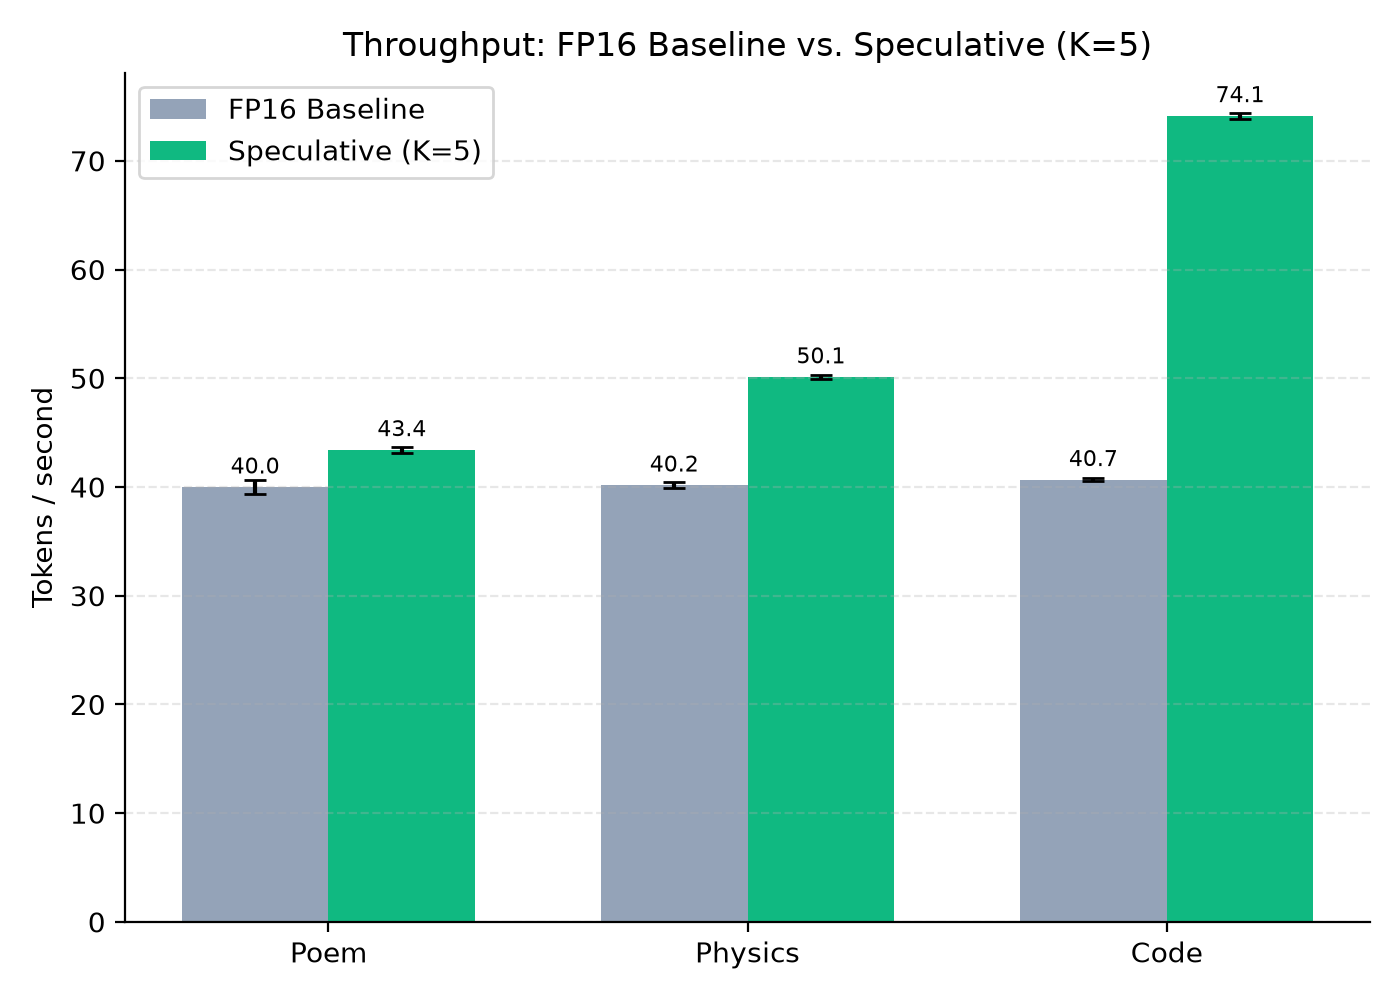
\includegraphics[width=\linewidth]{assets/throughput_baseline_vs_speculative.png}
\caption{Throughput}
\label{fig:throughput}
\end{subfigure}
\hfill
\begin{subfigure}{0.48\textwidth}
\centering
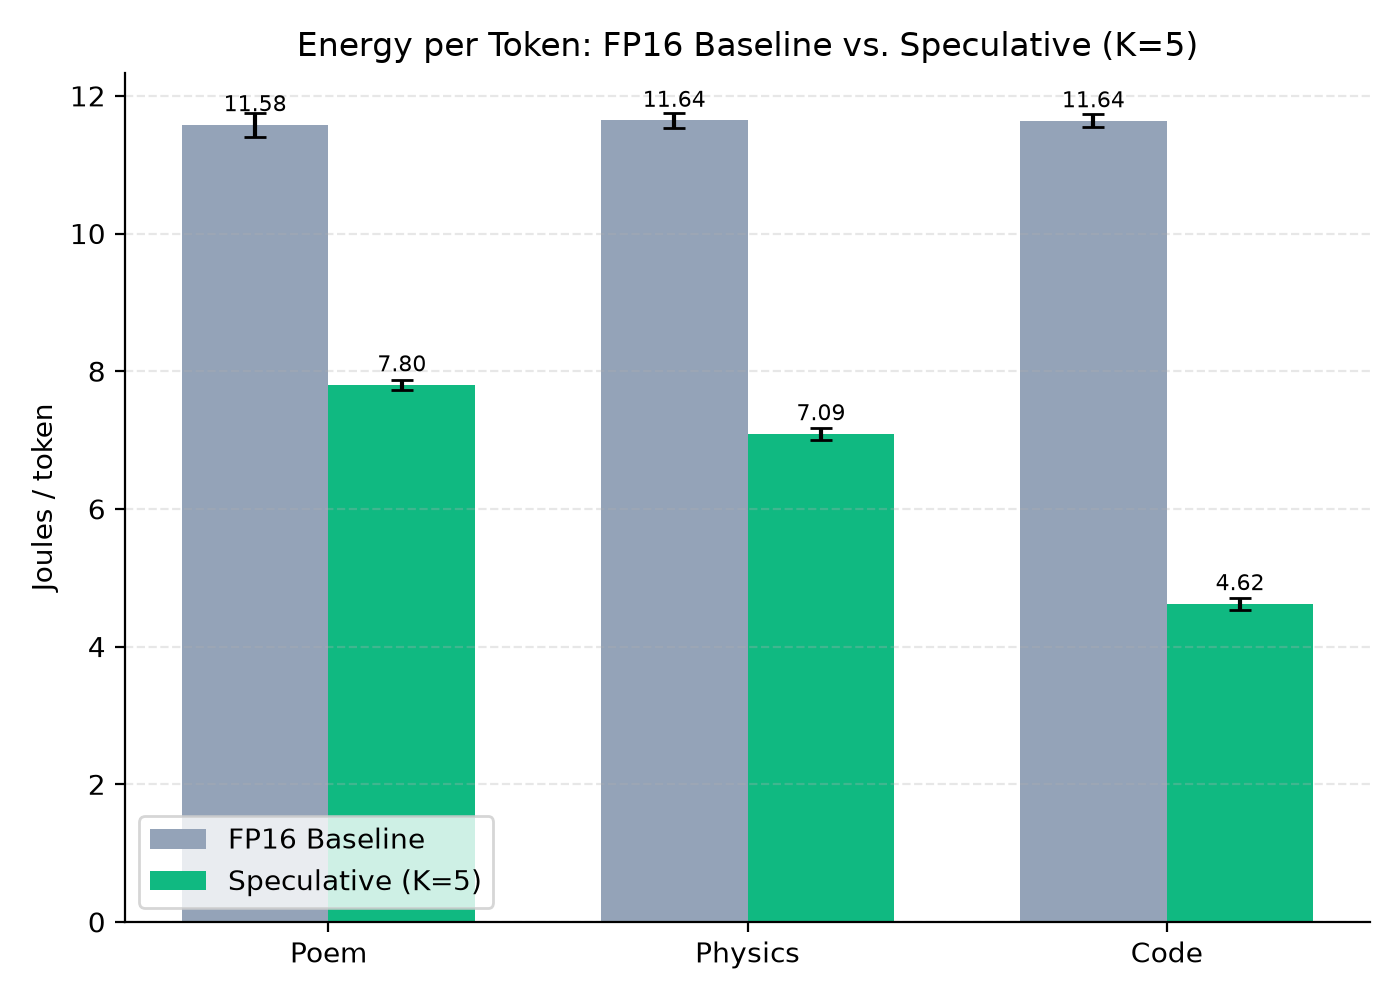
\includegraphics[width=\linewidth]{assets/energy_per_token_baseline_vs_speculative.png}
\caption{Energy per token}
\label{fig:energy}
\end{subfigure}
\caption{FP16 baseline vs. fixed-$K{=}5$ speculative decoding, per prompt (N=10 trials/prompt, error bars show $\pm 1$ std. dev.). Gains are smallest on the least predictable content (Poem) and largest on the most predictable (Code).}
\label{fig:throughput_energy}
\end{figure*}

\subsection{Speedup and energy reduction scale with acceptance rate}

Figure~\ref{fig:speedup_accept} shows speedup tracking draft acceptance
rate across the three prompts, consistent with the mechanism's expected
behavior: more predictable continuations (code) allow the scout to
correctly anticipate more tokens per cycle, directly translating to fewer
expensive target forward passes.

\begin{figure}[t]
\centering
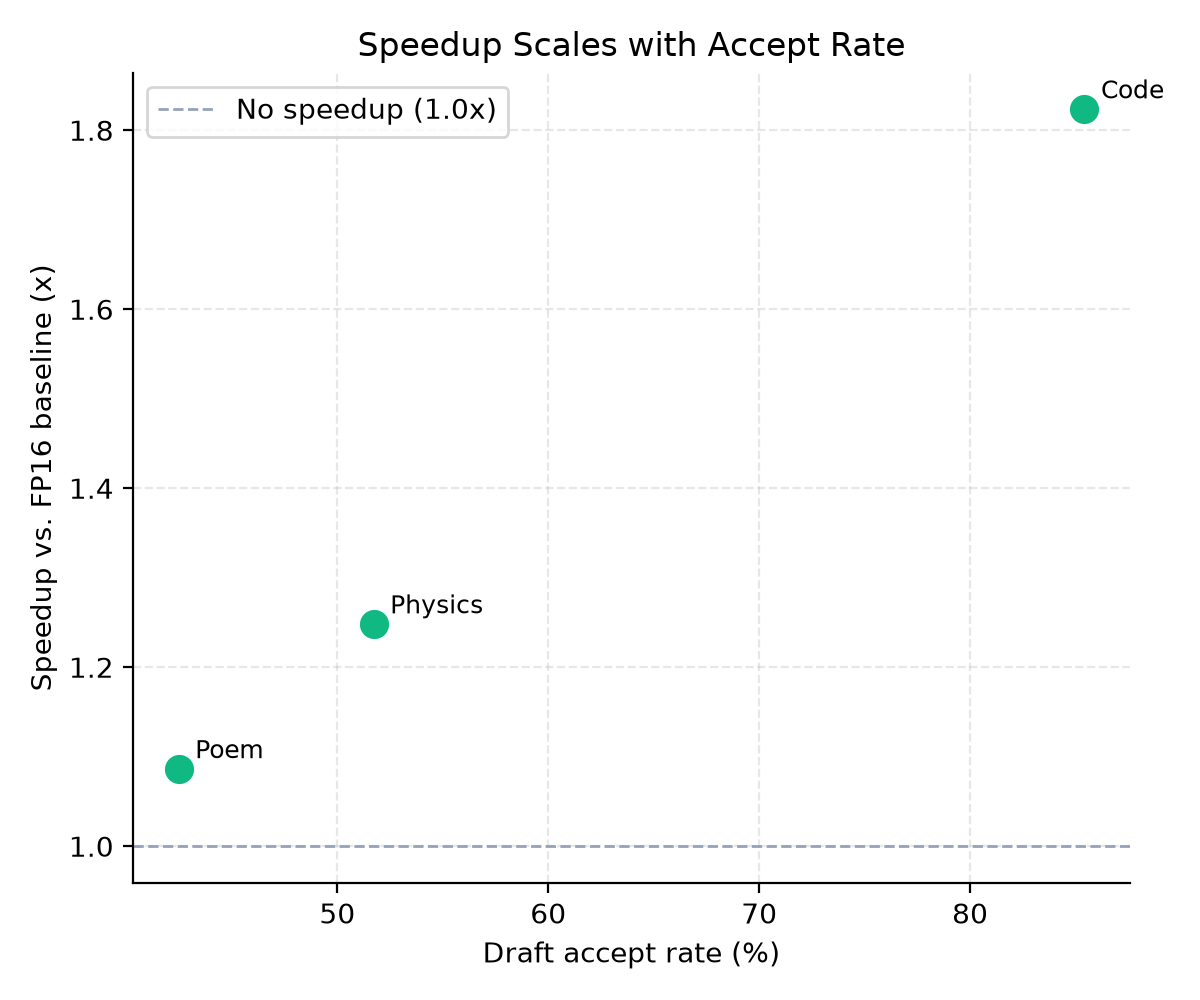
\includegraphics[width=0.9\linewidth]{assets/speedup_vs_accept_rate.png}
\caption{Speedup vs. FP16 baseline as a function of draft accept rate, across the three prompts. The relationship is monotonic and consistent with the mechanism's expected behavior.}
\label{fig:speedup_accept}
\end{figure}

\section{Discussion and Limitations}

\subsection{Absolute throughput is not production-representative}

As noted in Methodology, neither arm of this comparison uses KV-caching.
A production serving stack with proper cache reuse would show substantially
higher absolute throughput in both arms; we have not yet validated
fixed-$K$ speculative decoding's behavior under a cached, production-style
serving loop, and consider this the primary remaining gap before these
results can inform a deployment decision.

\subsection{Single-request, single-GPU scope}

All results in this paper are single-request (batch size 1) measurements
on a single consumer GPU. Behavior under batched, multi-request serving --
where the entropy-gated dynamic variant may plausibly outperform this
fixed-$K$ approach, per precedent in AdaEDL and SGLang -- is untested and
out of scope for this paper.

\subsection{Reproducibility}

All code, raw telemetry (JSON/CSV), and the scripts used to generate every
figure and table in this paper are available at
\url{https://github.com/Creepybits/sdsie-fixed-k5-speculative-decoding}
under an Apache-2.0 license. Reported numbers are directly traceable to
\texttt{telemetry/academic\_validation\_results.json}, generated by
\texttt{benchmark\_ablation.py} in that repository.

\section{Conclusion}

Fixed-$K{=}5$ speculative decoding, with an exact lossless verification
scheme, produces measurable and reproducible throughput and energy gains
on real consumer GPU hardware, scaling with output predictability, with
zero loss of output fidelity. We report this as a validated, narrow result,
distinct from and not dependent on the more experimental entropy-gated
dynamic mechanism under investigation elsewhere in the parent project.

\bibliographystyle{IEEEtran}
\begin{thebibliography}{9}

\bibitem{leviathan2023fast}
Y. Leviathan, M. Kalman, and Y. Matias,
``Fast Inference from Transformers via Speculative Decoding,''
\emph{Proc. 40th Int. Conf. Machine Learning (ICML)}, 2023.

\bibitem{chen2023accelerating}
C. Chen, S. Borgeaud, G. Irving, J.-B. Lespiau, L. Sifre, and J. Jumper,
``Accelerating Large Language Model Decoding with Speculative Sampling,''
arXiv:2302.01318, 2023.

\bibitem{adaedl2024}
Qualcomm AI Research,
``AdaEDL: Adaptive Entropy-based Dynamic Layer for Efficient Speculative Decoding,''
arXiv:2410.18351, 2024.

\end{thebibliography}

\end{document}
